\documentclass[10pt,hyperref={CJKbookmarks=true},xcolor=dvipsnames,aspectratio=169]{beamer}
\usetheme[navigation]{UMONS}
\usepackage[utf8]{inputenc}
\usepackage{verbatim}
\usepackage{ctex}

\title[国际经济学]{国际经济学}
\subtitle{国际收支理论:货币分析法}
\author{鲁晓东}
\institute[]{%
	岭南学院\hspace{2em}中山大学
	\\[4ex]
	
\includegraphics[height=8ex]{fig/lingnanlogo}\hspace{2em}%
	
\includegraphics[height=8.5ex]{fig/sysu}
}
%------------section前展示一页----------
\AtBeginSection[] {     
	\begin{frame}        
	\tableofcontents[currentsection,hideallsubsections]    
\end{frame} 
}

%-------------subsection也展示一下----------
\AtBeginSubsection[]{

\frame<beamer>{ 
	
	\frametitle{Outline}   
	
	\tableofcontents[currentsection,currentsubsection] 
	
}

}
%---------------------------

%-----------一段一闪现-------
%\beamerdefaultoverlayspecification{<+->}
%这个功能基本不用

\begin{document}
\maketitle


\begin{frame}
\frametitle{提纲}
\tableofcontents
\end{frame}				%生成提纲页

%-----------正文开始----------------------



\section{Motivation }
\begin{frame}{title}
\begin{itemize}[<+->]
	\item 汇率决定理论告诉我们,汇率的决定因素有哪些?
	\item 2018年第一季度我国经常账户录得逆差,引发市场对于汇率贬值压力加大的担忧。
	\item 这背后的逻辑是什么?
	\item 人民币“迟迟不肯破七”,这和中国的出口有关系吗?
	\item 为什么会有“贬值保出口”的说法,这背后的逻辑又是什么?
\end{itemize}
\centering
\includegraphics[scale=0.35]{fig/boptheory/ca}
\end{frame}



\section{The Multipliers Approach to the BOP}
\begin{frame}{OPEN ECONOMY MULTIPLIERS}

\begin{itemize}
	\item \textit{\textcolor{red}{John Maynard Keynes }}in his classic work
	\textit{\textcolor{blue}{The General Theory of Employment, Interest
			and Money}} published in 1936 pioneered the use of multiplier analysis
	to examine the effects of changes in government expenditure and investment
	on output and employment.
	\item It was not long, however, before the ideas of Keynes’ work were applied
	to an analysis of open economies, most notably by \textit{\textcolor{blue}{Fritz
			Machlup (1943)}}.
	\begin{figure}
		
		
		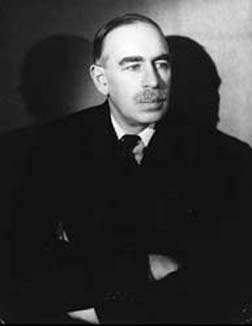
\includegraphics[scale=0.3]{fig/boptheory/lec08-9.JPG}
\includegraphics[scale=0.4]{fig/boptheory/lec08-8.JPG}
		
	\end{figure}
	
\end{itemize}
\end{frame}

\begin{frame}{The assumptions underlying basic multiplier analysis}

\begin{enumerate}
\item Both domestic prices and the exchange rate are fixed; 
\item The economy is operating at less than full employment so that increases
in demand result in an expansion of output;
\item The authorities adjust the money supply to changes in money demand
by pegging the domestic interest rate. 

\begin{enumerate}
	\item There is\textbf{\textcolor{blue}{{} no inflation resulting from the
			money supply}} expansion because it is merely a response to the increase
	in money demand.
\end{enumerate}
\end{enumerate}
\end{frame}

\begin{frame}[allowframebreaks]{Benchmark Derivation}

\begin{itemize}
\item The starting point
\[
Y=C+I+G+X-M
\]

\item taxes are proportional to income: $T=tY$
\item Domestic consumption is partly autonomous and partly determined by
the level of disposable national income: $C=C_{a}+c(1-t)Y$

\begin{itemize}
\item $C_{a}$ is autonomous consumption and $c$ is the marginal propensity
to consume
\end{itemize}
\item Import expenditure is assumed to be partly autonomous and partly a
positive function of the level of domestic income: $M=M_{a}+mY$

\begin{itemize}
\item $Ma$ is autonomous import expenditure and $m$ is the marginal propensity
to import
\end{itemize}
\item Rearrange, we abtain:
\end{itemize}

\begin{center}
$Y=C_{a}+c(1-t)Y+I+G+X-M_{a}-mY$
\par\end{center}


\[
Y[1\text{−}c(1\text{−}t)+m]=C_{a}+I+G+X\text{−}M_{a}
\]


\[
Y=\frac{1}{1-c(1-t)+m}\left(C_{a}+I+G+X\text{−}M_{a}\right)
\]

\end{frame}

\begin{frame}{Various Multiplers I}

\begin{itemize}
\item Above equation can be transformed into difference form to yield:
\end{itemize}

\begin{center}
$dY=\frac{1}{1-c(1-t)+m}\left(dC_{a}+dI+dG+dX\text{−}dM_{a}\right)$
\par\end{center}
\begin{itemize}
\item The government expenditure multiplier
\end{itemize}

\[
\frac{dY}{dG}=\frac{1}{1-c(1-t)+m}>0
\]

\begin{itemize}
\item Since {[}$1-c(1-t)+m${]} is less than unity, an increase in government
expenditure will result in an even greater increase in national income.
\end{itemize}
\end{frame}

\begin{frame}{Numerical Example}

\begin{exampleblock}{Assume that the marginal propensity to consume is 0.8, the tax rate
is 25\% of income, i.e. t = 0.25, and the marginal propensity to import
is 0.3. The effect of an increase in government expenditure of £100
million on national income is given by:}

\end{exampleblock}
\[
dY=\frac{1}{1-c(1-t)+m}dG=\frac{1}{1-0.8\left(1-0.25\right)+0.30}100m
\]


\[
=1.4286\times100m=142.86m
\]

\end{frame}

\begin{frame}{Various Multiplers II}

\begin{itemize}
\item The foreign trade or export multiplier

\begin{itemize}
\item the multiplier effect of an increase in exports on national income
is identical to that of an increase in government expenditure.
\[
dY/dX=1/[1\text{−}c(1\text{−}t)+m]
\]

\end{itemize}
\item The current account multipliers

\begin{itemize}
\item the effects of an increase in government expenditure and of exports
on the current account (CA) balance
\[
CA=X-M=X-M_{a}-\frac{m}{1-c(1-t)+m}\left(C_{a}-M_{a}+I+G+X\right)
\]

\end{itemize}
\item we can derive that:
\end{itemize}

\[
dCA/dG=\text{−}m/[1\text{−}c(1\text{−}t)+m]<0
\]

\begin{theorem}
an increase in government spending leads to a deterioration of the
current account balance
\end{theorem}

\end{frame}

\begin{frame}{Various Multiplers III}

\begin{itemize}
\item the effect of an increase in exports on the current balance
\end{itemize}

\[
\frac{dCA}{dX}=\text{1−}\frac{m}{1\text{−}c(1\text{−}t)+m}=\frac{1\text{−}c(1\text{−}t)+m}{1\text{−}c(1\text{−}t)+m}-\frac{m}{1\text{−}c(1\text{−}t)+m}
\]



\begin{block}{Since$(1-c(1-t))/[1-c(1-t)+m)]$ is less than unity, an increase in
exports leads to an improvement in the current balance that is less
than the original increase in exports.}

\end{block}
\end{frame}

\begin{frame}{Main Conclusions}

\begin{itemize}
\item Keynesian income effects are an essential part of balance of payments
analysis
\item Downsides

\begin{itemize}
\item Analysis of macroeconomic fluctuations for an open economy requires
consideration of what is happening in foreign economies
\item The foreign trade multiplier analysis deals with \textbf{\textcolor{blue}{what
happens to the balance of payments when income changes, assuming that
prices are held constant}}.
\end{itemize}
\end{itemize}
\end{frame}



\section{The Elasticity Approach to the BOP}
\begin{frame}{Introduction}

\begin{itemize}
\item We will investigate the relationship between the exchange rate and
the balance of payments
\item More Specifically, Whether will the fluctuation in exchange rate impact
the balance of payments
\item There are two traditional Models were designed to tackle one of the
most important questions in international economics

\begin{itemize}
\item Elasticity approach——局部均衡模型
\item Absorption approach——一般均衡模型
\end{itemize}
\end{itemize}
\end{frame}

\begin{frame}{Intellegence History of Elasticity Approach to the BOP}

\begin{itemize}
\item The analysis was pioneered by \textbf{\textcolor{blue}{Alfred Marshall
(1923)}} and\textbf{\textcolor{blue}{{} Abba Lerner (1944)}}, and later
extended by \textbf{\textcolor{blue}{Joan Robinson (1937) }}and \textbf{\textcolor{blue}{Fritz
Machlup (1939)}}
\item Basic Assumptions:

\begin{itemize}
\item The supply elasticities for the domestic export good and foreign import
good are \textbf{\textcolor{blue}{perfectly elastic}}
\item These assumptions mean that domestic and foreign prices are fixed
\item Changes in relative prices are caused by changes in the nominal exchange
rate
\begin{figure}
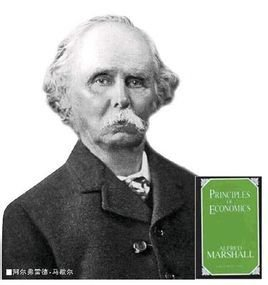
\includegraphics[scale=0.3]{fig/boptheory/lec08-10.JPG}

\includegraphics[scale=0.3]{fig/boptheory/lec08-11.JPG}

\end{figure}

\end{itemize}
\end{itemize}
\end{frame}

\begin{frame}{Elasticity Approach to the BOP}

\begin{itemize}
\item The central message of the elasticity approach is that there are two
direct effects of a devaluation on the current balance

\begin{itemize}
\item reduce a deficit
\item make the deficit worse than before
\end{itemize}
\item The current account balance is given by:
\end{itemize}

\[
CA=PX_{v}\text{−}SP^{*}M_{v}
\]

\begin{itemize}
\item where $P$ is the domestic price level, $X_{v}$ is the volume of
domestic exports, $S$ is the exchange rate (domestic currency units
per unit of foreign currency), $P^{*}$ is the foreign price level
and $M_{v}$ is the volume of imports
\end{itemize}
\end{frame}

\begin{frame}{Elasticities}

\begin{itemize}
\item In difference form equation
\end{itemize}

\[
dCA=dX\text{−}SdM\text{−}MdS
\]


\[
\frac{dCA}{dS}=\frac{dX}{dS}-S\frac{dM}{dS}-M\frac{dS}{dS}
\]

\begin{itemize}
\item Define

\begin{itemize}
\item \textbf{\textcolor{blue}{the price elasticity of demand for exports}}
$\eta_{x}=-\frac{dX/X}{dS/S}$, so that \textrm{$dX=-\frac{X\eta_{x}dS}{S}$}

\item \textbf{\textcolor{red}{the price elasticity of demand for imports}}
$\eta_{m}=\frac{dM/M}{dS/S}$, so that \textrm{$dM=\frac{M\eta_{m}dS}{S}$}
\end{itemize}
\end{itemize}
\end{frame}

\begin{frame}{Marshall–Lerner condition}

\begin{itemize}
\item Assuming that we initially have balanced trade, $X/SM=1$
\end{itemize}

\[
\frac{dCA}{dS}=M\left(\eta_{x}+\eta_{m}-1\right)
\]

\begin{itemize}
\item If $\eta_x+\eta_m>1$, a devaluation will improve the current account
\item If $\eta_x+\eta_m<1$,a devaluation will lead to a deterioration of
the current account
\end{itemize}
\end{frame}

\begin{frame}{Effects of devaluation}

\begin{itemize}
\item The price effect

\begin{itemize}
\item exports become cheaper measured in foreign currency
\item Imports become more expensive measured in the home currency
\end{itemize}
\item The volume effect

\begin{itemize}
\item exports become cheaper should encourage an increased volume of exports,
and the fact that imports become more expensive should lead to a decreased
volume of imports.
\end{itemize}
\item \textbf{\textcolor{blue}{The net effect depends upon whether the price
or volume effect dominates.}}
\end{itemize}
\end{frame}

\begin{frame}{Extension of Marshall-lerner Condition}

\begin{itemize}
\item If we assume that supply elasticities of exports and imports of less
than infinity(标准条件假定供给弹性无穷大).
\item \textbf{\textcolor{blue}{Stern (1973)}} has shown that a more complicated
condition needs to be satisfied
\end{itemize}

\[
\frac{\varepsilon_{x}(\eta_{x}-1)}{\varepsilon_{x}+\eta_{x}}+\frac{\eta_{m}(\varepsilon_{m}-1)}{\varepsilon_{m}+\eta_{m}}>0
\]

\begin{itemize}
\item where $\varepsilon_{x}$ is the domestic supply elasticity of the
export good and $\varepsilon_{m}$ is the foreign supply elasticity
for its export good
\item The effect of less-than-infinite supply price elasticities is to make
the required demand elasticities less stringent(使得原来的条件被放松,没有之前那么严格)
\end{itemize}
\end{frame}

\begin{frame}{Empirical Evidence For Developed Countries}


\begin{figure}


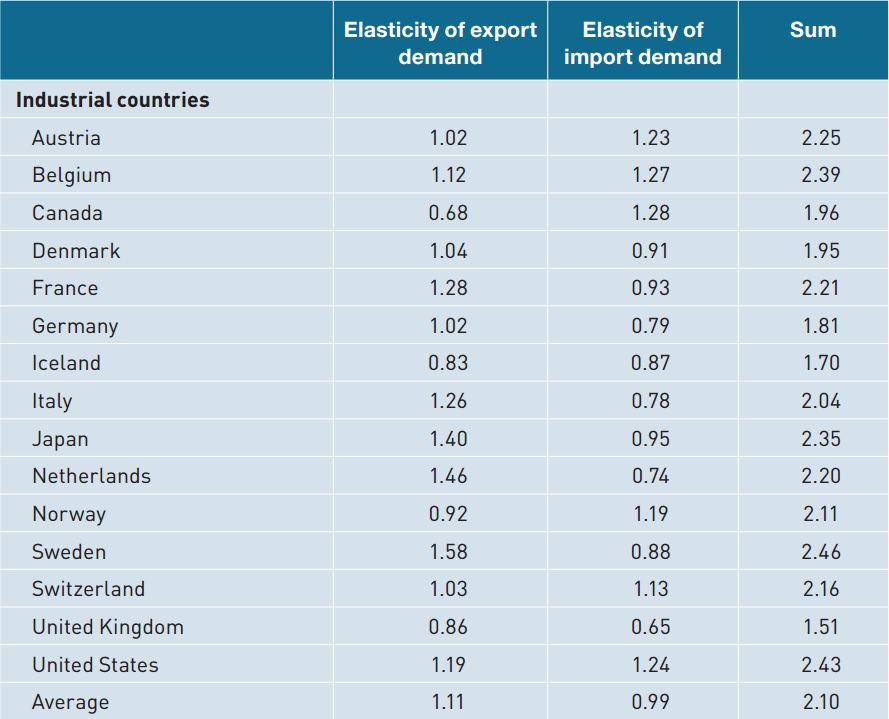
\includegraphics[scale=0.35]{fig/boptheory/lec08-12.JPG}

\end{figure}

\end{frame}

\begin{frame}{J Curve}


\begin{columns}[onlytextwidth]
\begin{column}{0.4\textwidth}
\begin{itemize}
\item Elasticities are lower in the short run than in the long run, in which
case the Marshall–Lerner conditions may not hold in the short run
but may hold in the medium to long run.
\item This lead to the phenomenon of what is popularly known as the \textbf{\textcolor{red}{J-curve
effect}}
\end{itemize}

\end{column}
\begin{column}{0.6\textwidth}
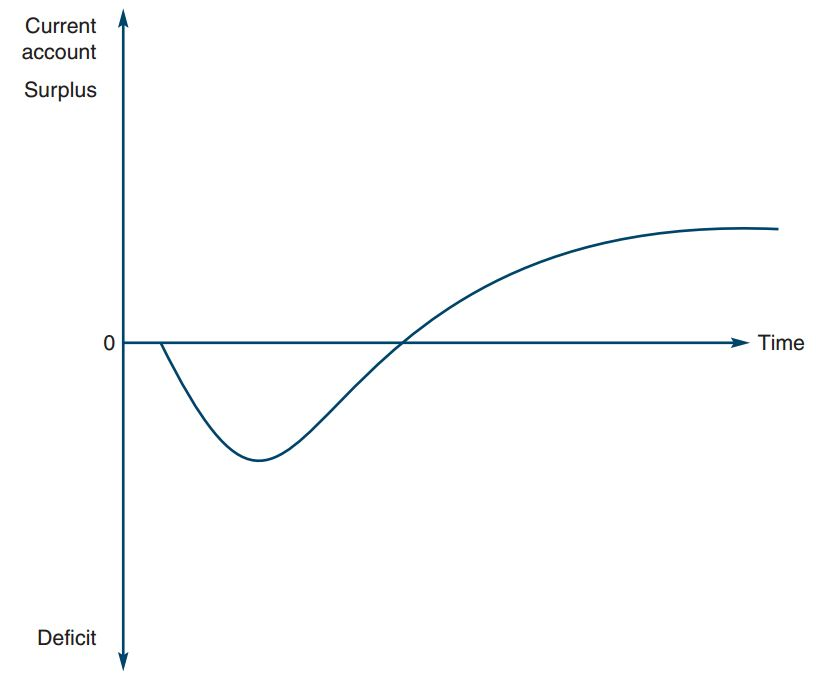
\includegraphics[width=0.9\columnwidth]{fig/boptheory/lec08-13}
\end{column}
\end{columns}

\end{frame}

\begin{frame}{Explanation on J curve effect}

\begin{itemize}
\item A time lag in consumer responses.
\item A time lag in producer responses.
\item Imperfect competition. 
\end{itemize}
\end{frame}

\begin{frame}{PASS-THROUGH EFFECT OF A DEPRECIATION OR APPRECIATION}

\begin{itemize}
\item The preceding analysis assumed that a 10\% depreciation/devaluation
will lead to a rise in price of imports by 10\%.
\item Pass Through

\begin{itemize}
\item the extent to which a 1\% depreciation (appreciation) leads to a rise
(fall) in import prices. 
\item the elasticity of exchange rate pass-through
\end{itemize}
\item Causes

\begin{itemize}
\item Imperfect competition
\end{itemize}
\item Empirically, there is only a partial pass-through effect on the price
of imports in the short run
\item This effect will be to dampen the size and complicate the dynamics
and timing of the J-curve effect.
\end{itemize}
\end{frame}

\begin{frame}{Insensitivity of export to exchange Rate: My Estimation}




\begin{columns}[onlytextwidth]
\begin{column}{0.4\textwidth}
\begin{itemize}
\item One of the central puzzles in international macroeconomics is why
large movements in exchange rates have small effects on the prices
of internationally traded goods.
\item Large exporters are simultaneously large importers
\end{itemize}

\end{column}
\begin{column}{0.6\textwidth}
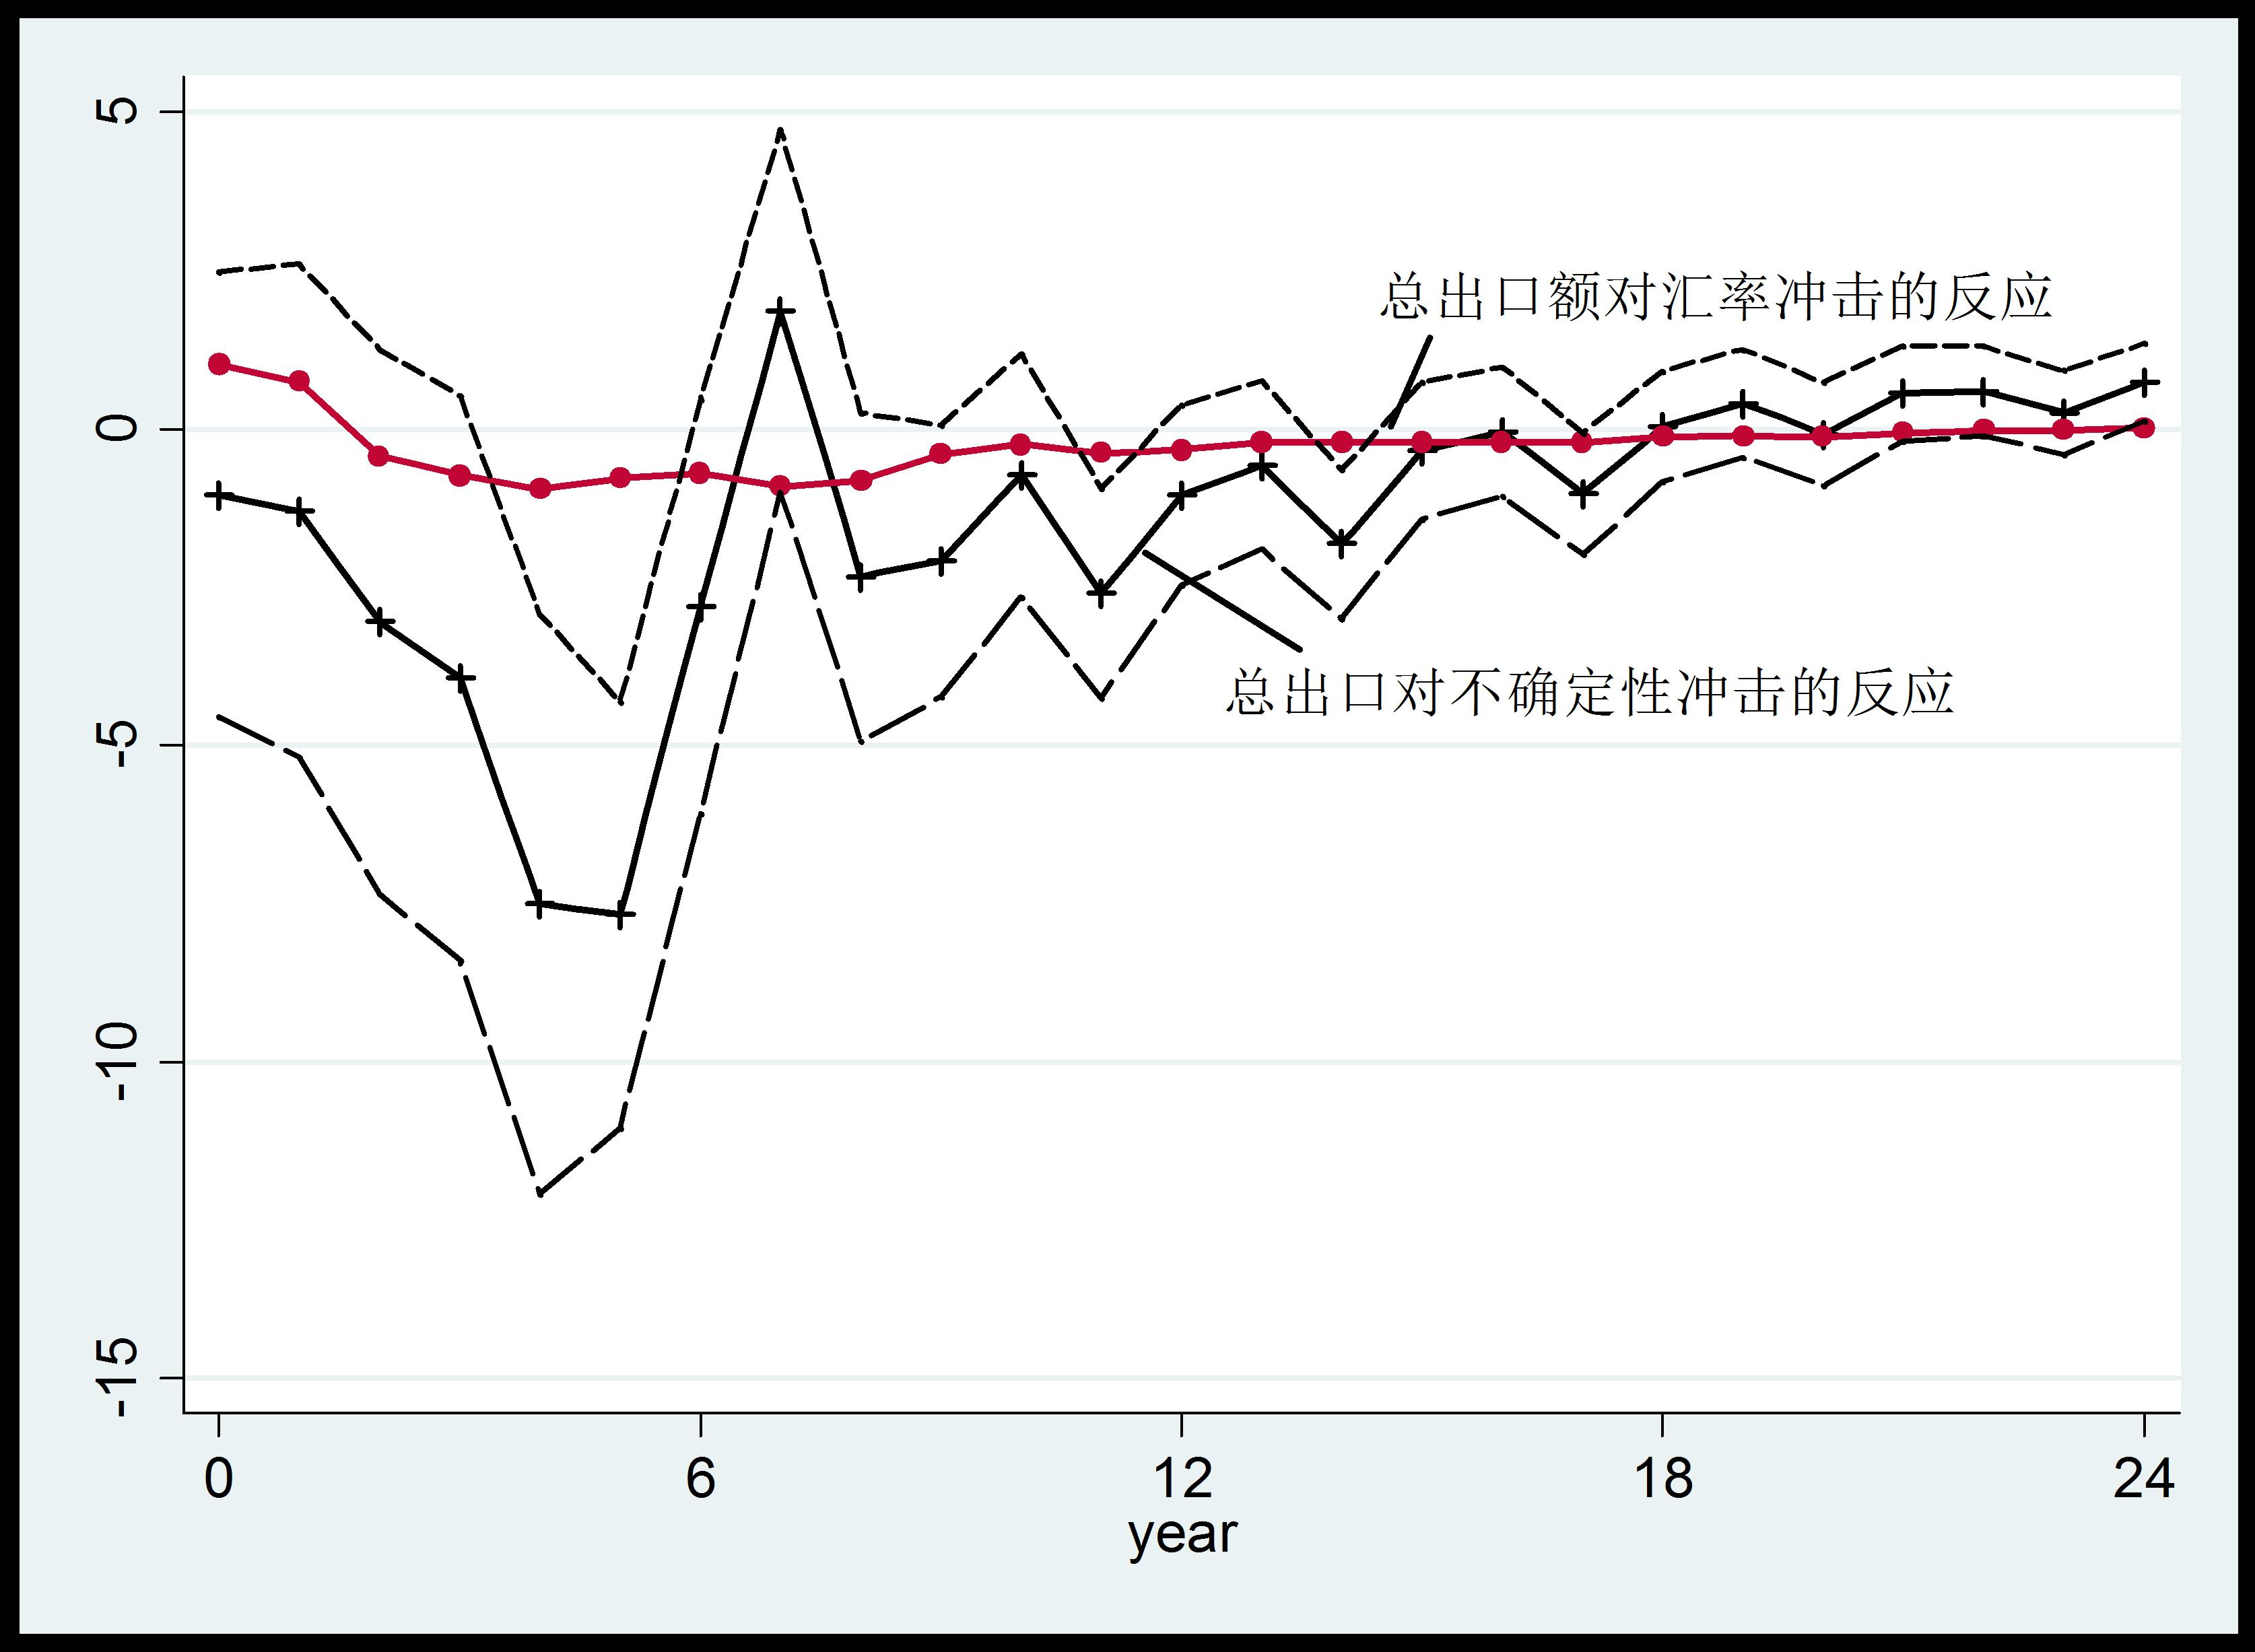
\includegraphics[width=\columnwidth]{fig/boptheory/lec08-37}
\end{column}
\end{columns}

\end{frame}



\section{The Absorption Approach to the BOP}
\begin{frame}{Intellegence History}

\begin{itemize}
\item Caveat of Elasticity approach

\begin{itemize}
\item Assuming that all other things are equal
\item However, changes in export and import volumes will by definition have
implications for national income
\end{itemize}
\item \textbf{\textcolor{blue}{Alexander (1952) }}is one of the most important
papers to evaluate this effect

\begin{itemize}
\item a current account imbalance can be viewed as the difference between
domestic output and domestic spending (absorption)
\end{itemize}
\end{itemize}
\end{frame}

\begin{frame}[allowframebreaks]{The Absorption Approach}

\begin{itemize}
\item Taking the equation for national income:
\end{itemize}

\[
Y=C+I+G+X\text{−}M
\]

\begin{itemize}
\item Domestic absorption: $A=C+I+G$
\end{itemize}

\[
CA=X\text{−}M=Y\text{−}A
\]


\[
dCA=dY-dA
\]

\begin{itemize}
\item The above equation implies is that the effects of a devaluation on
the current balance will depend upon how it affects national income
relative to how it affects domestic absorption. 
\item Absorption can be divided up into two parts

\begin{itemize}
\item a rise in income will lead to an increase in absorption which is determined
by the marginal propensity to absorb, denoted by $a$
\item there will also be a ‘direct effect’ on absorption, which is all the
other effects on absorption resulting from devaluation, denoted by
$A_{d}$. 可以理解为贬值对商品价格的影响
\item the change in total absorption dA, is given by:
\end{itemize}

\[
dA=adY+dA_{d}
\]


\end{itemize}

\[
dCA=(1\text{−}a)dY\text{−}dA_{d}
\]

\begin{block}{结论}
	贬值对于经常账户的影响取决于三个方面:改变边际吸收倾向$a$,改变国民收入水平$4dY$,影响直接吸收。
\end{block}



\end{frame}

\begin{frame}{Effects of devaluation on national income}

\begin{itemize}
\item Employment effect.

\begin{itemize}
\item Depends on whether it is full employment and MLC
\item if the economy is at a position of full employment, an increase in
income is not possible. 
\end{itemize}
\item Terms of trade effect

\begin{itemize}
\item A deterioration in the terms of trade represents a loss of real national
income.
\end{itemize}
\end{itemize}

\[
\frac{Price of export}{Price of import}=\frac{P}{SP^{*}}
\]



\end{frame}

\begin{frame}{Effects of devaluation on marginal	propensity to absorb}

\begin{itemize}
	\item Even if income rises overall, it is still not clear what the implications of a rise in
	income are for the current account, as this will depend upon the value of the marginal	propensity to absorb
	
	\item Is it always less than Unity?
	\item  Although
	one may think that the marginal propensity to absorb will be less than unity this
	need not be the case
	\item If $a>1$, How to make it reasonable?
	
\end{itemize}
\end{frame}

\begin{frame}{Effects of devaluation on direct absorption}

\begin{itemize}
\item let us assume that the net effect of a devaluation on income is zero
\item This being the case, we must consider the effect of the devaluation
on direct absorption.
\item possible ways in which a devaluation can be expected to impact upon
direct absorption.

\begin{itemize}
\item Real balance effect实际余额效应
\item Income redistribution effect收入再分配效应
\item Money illusion effect货币幻觉效应
\item Expectational effects预期效应
\item Laursen–Metzler effect
\end{itemize}
\end{itemize}
\end{frame}

\begin{frame}{Real balance effect}

\begin{itemize}
\item the relationship between prices and the demand to hold ream money
balances
\item Algebraically a money demand function can be expressed as:
\end{itemize}

\[
M/P_{I}=k
\]

\begin{itemize}
\item where $k$ is some constant and $P_{I}$ is an aggregate price index
defined as:
\end{itemize}

\[
P_{I}=\alpha P+(1\text{−}\alpha)SP*
\]

\begin{itemize}
\item where $\alpha$ is the percentage of expenditure on domestic goods,
$P$ is the price of the domestic good, $P*$ is the price of the
foreign import good, and $S$ is the exchange rate defined as domestic
currency units per unit of foreign currency.\end{itemize}
\begin{block}{A devaluation (rise in S) will reduce direct absorption.}



\end{block}
\end{frame}

\begin{frame}{Income redistribution effect}



\begin{itemize}
\item redistributes income between those with a low marginal propensity
to absorb and those with a high marginal propensity to absorb

\begin{itemize}
\item The rise in the general price index will tend to change the real income
of those with fixed incomes and those with variable incomes in different
ways
\item A devaluation often leads to an improvement of company profits through
increased sales in export and import-competing industries
\item There may be considerable income adjustments within groups of companies
and workers. 
\end{itemize}
\end{itemize}
\end{frame}

\begin{frame}{Money illusion effect}

\begin{itemize}
\item Price changed, but consumers suffer ‘money illusion’ and buy exactly
the same bundle of goods as before
\item they are actually spending more on direct absorption than before
\item However, the money illusion effect may work in reverse
\end{itemize}
\end{frame}

\begin{frame}{Expectational effects}

\begin{itemize}
\item Economic agents regard the price rises induced by devaluation as likely
to spark further price rises. This would lead to an increase in direct
absorption which would worsen the balance of payments.
\item However, against this it can be argued that inflationary expectations
may reduce investment which lowers direct absorption.
\end{itemize}
\end{frame}

\begin{frame}{Laursen–Metzler effect}

\begin{itemize}
\item Laursen and Metzler (1950) noted that the deterioration in the terms
of trade following a devaluation will have two effects on absorption:

\begin{itemize}
\item an income effect 
\item a substitution effect.
\end{itemize}
\item Hence, the effects of a devaluation on direct absorption are \textbf{\textcolor{red}{ambiguous}}.
\item Policy Implication

\begin{itemize}
\item raising domestic income relative to domestic absorption will improve
the current balance. 
\item a devaluation is more likely to succeed if it is accompanied by economic
policy measures that concentrate on raising income while constraining
absorption.
\end{itemize}
\end{itemize}
\end{frame}

\begin{frame}{Synthesis of Elasticity Approach and Absorption Approach}

\begin{itemize}
\item Distinctions

\begin{itemize}
\item the elasticity approach concentrating on price effects
\item the absorption approach concentrated on income effects
\end{itemize}
\item Complementarity

\begin{itemize}
\item The initial improvement in the current account has to be more pronounced
than in the absence of such income effects
\end{itemize}
\end{itemize}
\end{frame}



\section{The Monetary Approach to the BOP(Selective)}
\begin{frame}{Intellectual History}

\begin{itemize}
\item The monetary approach

\begin{itemize}
\item One of the most influential policy analyses of the balance of payments 
\item was pioneered by Marina \textbf{\textcolor{red}{Whitman (1975) }}and
\textbf{\textcolor{red}{Jacob Frenkel and Harry Johnson (1976)}}
\end{itemize}
\item fundamental basis of the monetary approach

\begin{itemize}
\item \textbf{\textcolor{blue}{BOP can only be explained by a disequilibrium
in the stock demand for and supply of money.}}
\end{itemize}
\item Assumptions

\begin{itemize}
\item stable money demand function
\item vertical aggregate supply schedule
\item purchasing power parity (PPP)
\end{itemize}
\end{itemize}
\end{frame}

\begin{frame}{Stable money demand function}


\begin{columns}[onlytextwidth]
\begin{column}{0.5\textwidth}
\begin{itemize}
\item the money demand function
\end{itemize}

\[
M_{d}=kPy\begin{array}{c}
,\end{array}where\begin{array}{c}
,\end{array}k>0
\]

\begin{itemize}
\item \textbf{\textcolor{red}{if we hold the money supply/money demand fi
xed and assume that k is a fixed parameter, the aggregate demand schedule
is a rectangular hyperbola given by AD1}}
\item \textbf{\textcolor{red}{at any given price level there is a rise in
real money balances which leads to increased aggregate demand.}}
\end{itemize}

\end{column}
\begin{column}{0.5\textwidth}
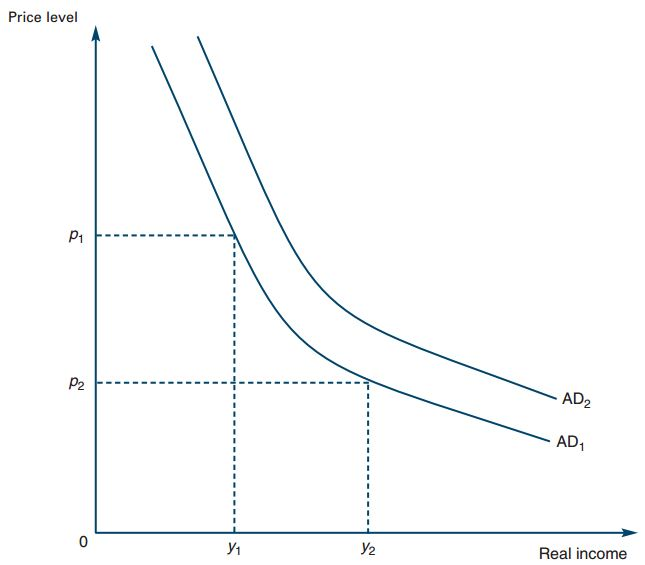
\includegraphics[width=\columnwidth]{fig/boptheory/lec08-14}
\end{column}
\end{columns}

\end{frame}

\begin{frame}{Vertical aggregate supply schedule}




\begin{columns}[onlytextwidth]
\begin{column}{0.4\textwidth}
\begin{itemize}
\item Wages are sufficiently flexible that they are constantly at the level
that equates the supply and demand for labour.
\item Rise in the domestic price level does not lead to an increase in domestic
output
\item Increase in y depends on technological advance.
\end{itemize}

\end{column}
\begin{column}{0.6\textwidth}
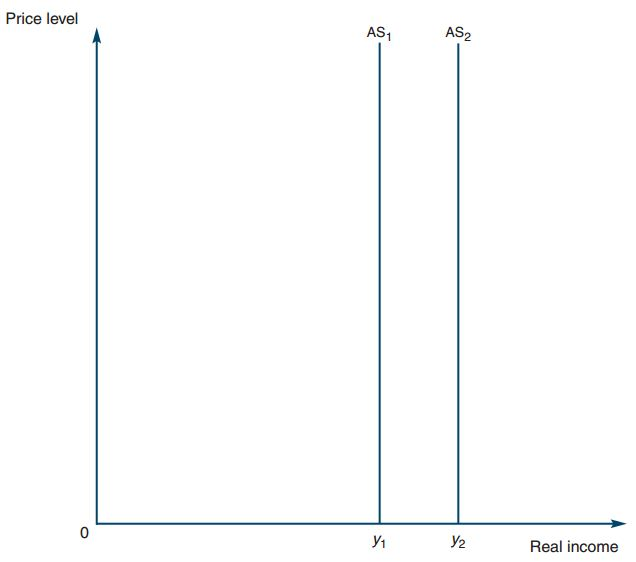
\includegraphics[width=0.8\columnwidth]{fig/boptheory/lec08-15}
\end{column}
\end{columns}

\end{frame}

\begin{frame}{PPP}




\begin{columns}[onlytextwidth]
\begin{column}{0.4\textwidth}
\begin{itemize}
\item purchasing power parity (PPP)
\end{itemize}

\[
S=\frac{P}{P^{*}}\begin{array}{c}
\end{array}that\begin{array}{c}
is\end{array},\begin{array}{c}
\end{array}P=SP^{*}>0
\]

\begin{itemize}
\item PPP schedule shows combinations of the domestic price level and exchange
rate which are compatible with PPP, given the foreign price level
P{*}. 
\end{itemize}

\end{column}
\begin{column}{0.6\textwidth}
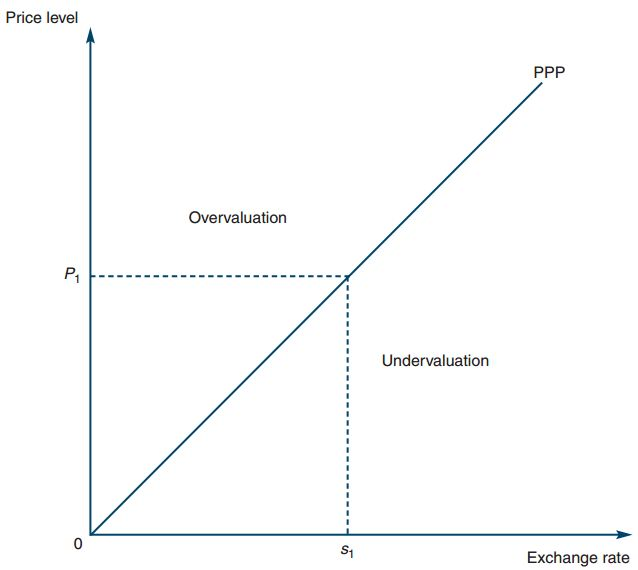
\includegraphics[width=0.9\columnwidth]{fig/boptheory/lec08-16}
\end{column}
\end{columns}

\end{frame}

\begin{frame}{Domestic Monetary Supply}




\begin{columns}[onlytextwidth]
\begin{column}{0.4\textwidth}
\begin{itemize}
\item The domestic monetary supply in the economy is made up of two components:
\end{itemize}

\[
M_{s}=D+R
\]

\begin{itemize}
\item The monetary base can come into circulation in one of two ways. 

\begin{itemize}
\item open-market operation (OMO)
\item foreign exchange operation (FXO) 
\end{itemize}
\end{itemize}

\end{column}
\begin{column}{0.6\textwidth}
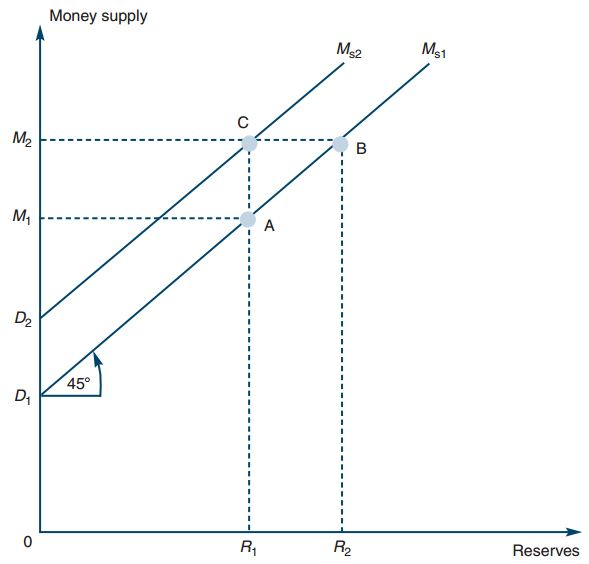
\includegraphics[width=0.8\columnwidth]{fig/boptheory/lec08-17}
\end{column}
\end{columns}

\end{frame}

\begin{frame}{Montetarist concept of BOP disequilibrium}

\begin{itemize}
\item The monetarists view balance of payments surpluses and deficits as
monetary flow due to stock disequilibrium in the money market. 
\end{itemize}

\[
M_{s}>M_{d}orM_{s}<M_{d}
\]

\begin{itemize}
\item Keynesians: top $\Rightarrow$ down

\begin{itemize}
\item Monetarists: bottom $\Rightarrow$ up
\end{itemize}
\item the overall balance of payments (BP) can be thought of as consisting
of the current account balance, the capital account balance and the
changes in the authorities’ reserves.
\end{itemize}

\[
BP=CA+K+dR=0
\]

\begin{itemize}
\item so that
\end{itemize}

\[
CA+K=\text{−}dR
\]





\end{frame}

\begin{frame}{Analytical Framework}


\begin{figure}
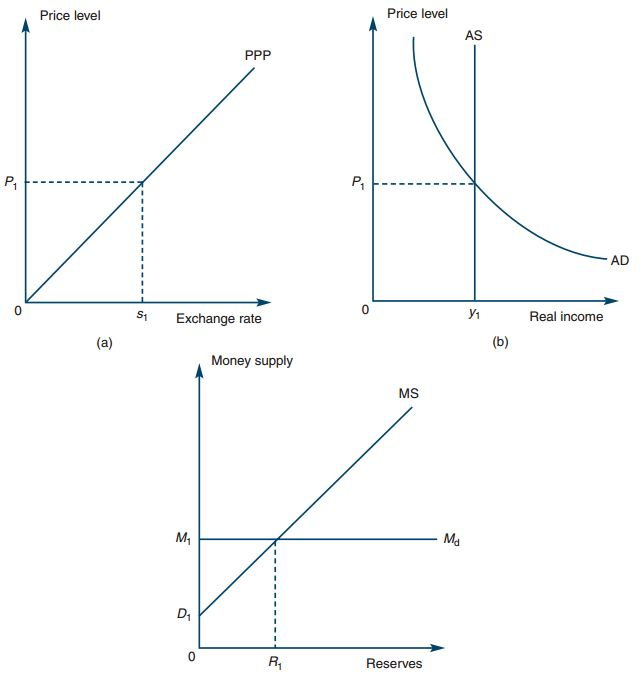
\includegraphics[scale=0.5]{fig/boptheory/lec08-18.JPG}

\end{figure}

\end{frame}

\begin{frame}{Shocks I: Devaluation}


\begin{figure}


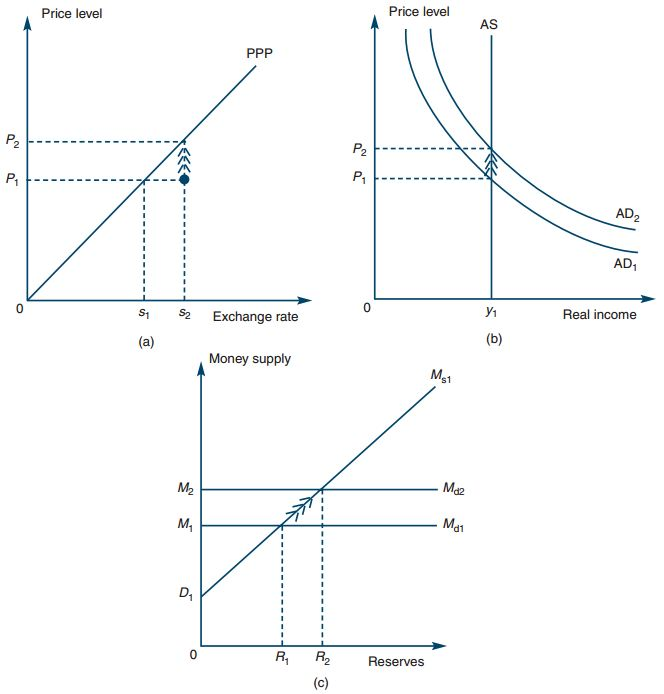
\includegraphics[scale=0.5]{fig/boptheory/lec08-19.JPG}
\end{figure}

\end{frame}

\begin{frame}{A Monetary Exchange Rate Equation}

\begin{itemize}
\item the exchange rate
\end{itemize}

\[
S=\frac{M_{s}/M_{s^{*}}}{ky/k^{*}y^{*}}
\]

\begin{itemize}
\item states that the exchange rate is determined by the relative supply
and demand for the different national money stocks. 
\end{itemize}
\end{frame}

\begin{frame}{Shock II: Money Supply Expansion under fixed exchange rate}
\begin{figure}


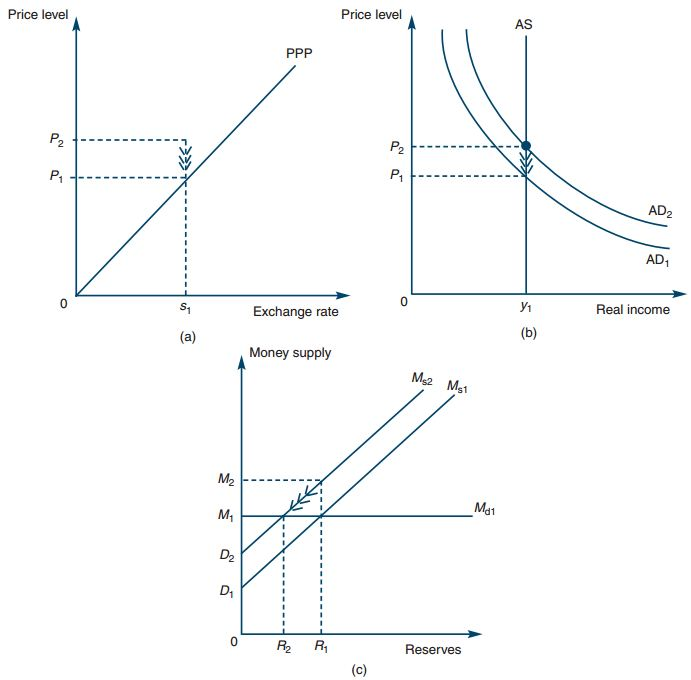
\includegraphics[scale=0.4]{fig/boptheory/lec08-20.JPG}

\end{figure}

\end{frame}

\begin{frame}{Shock II: Money Supply Expansion under floating exchange rate}


\begin{figure}


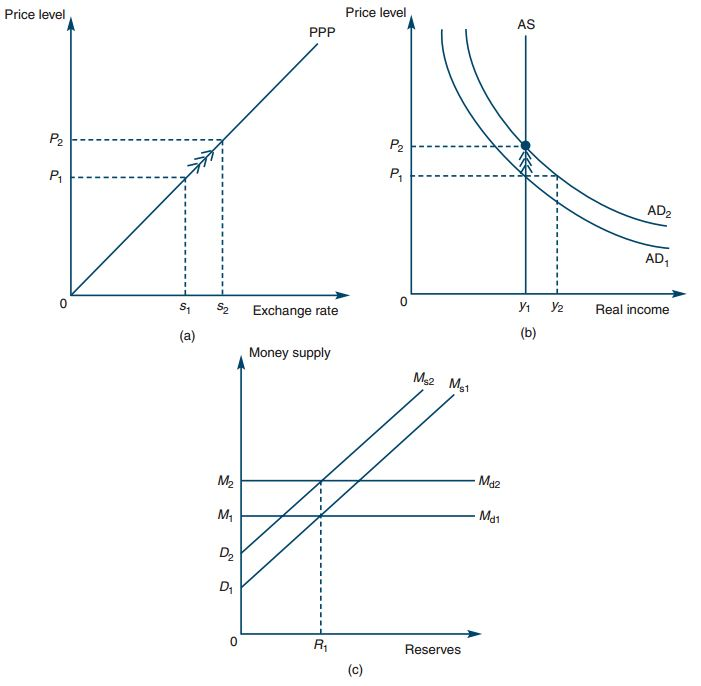
\includegraphics[scale=0.4]{fig/boptheory/lec08-21.JPG}
\end{figure}

\end{frame}

\begin{frame}{Shock III: Increase in income under fixied exchange rate}


\begin{figure}


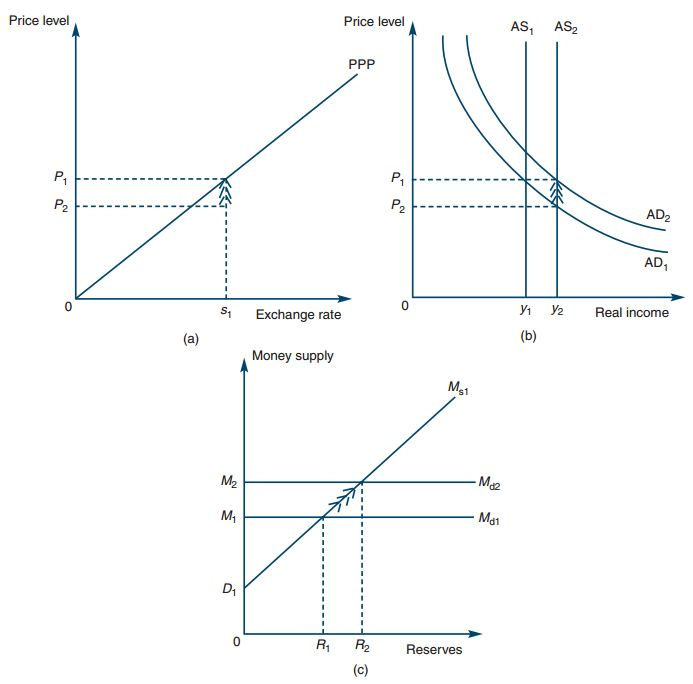
\includegraphics[scale=0.4]{fig/boptheory/lec08-22.JPG}

\end{figure}

\end{frame}

\begin{frame}{Shock III: Increase in income under floating exchange rate}


\begin{figure}


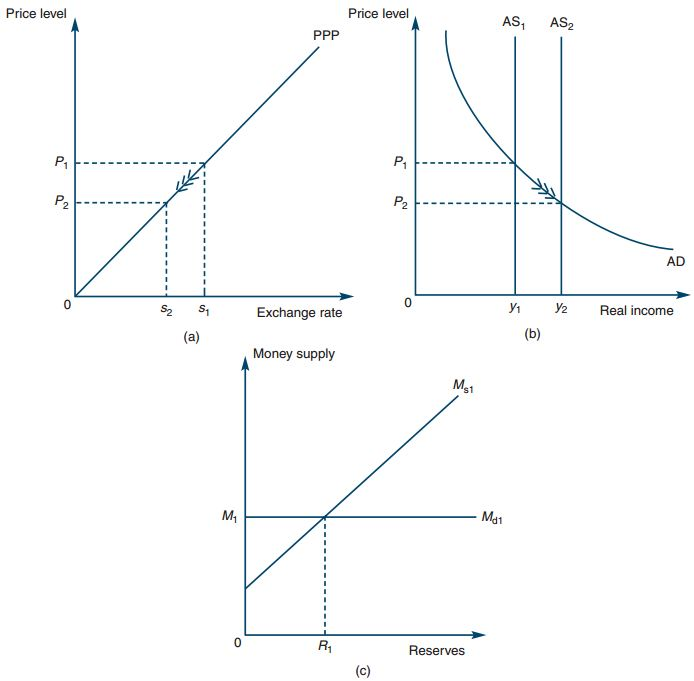
\includegraphics[scale=0.4]{fig/boptheory/lec08-23.JPG}

\end{figure}

\end{frame}

\begin{frame}{Shock IV: Increase in foreign Price under Fixed Exchange Rate}


\begin{figure}


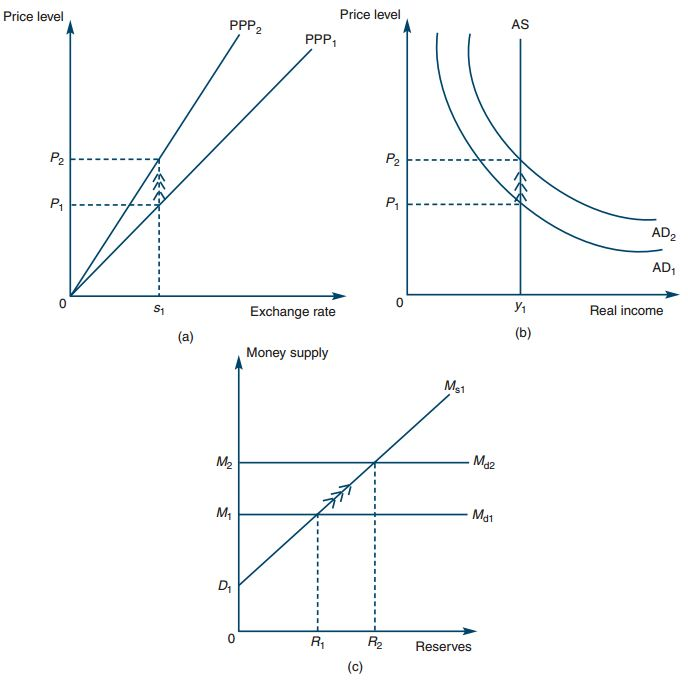
\includegraphics[scale=0.4]{fig/boptheory/lec08-24.JPG}

\end{figure}

\end{frame}

\begin{frame}{Shock IV: Increase in foreign Price under Floating Exchange Rate}


\begin{figure}


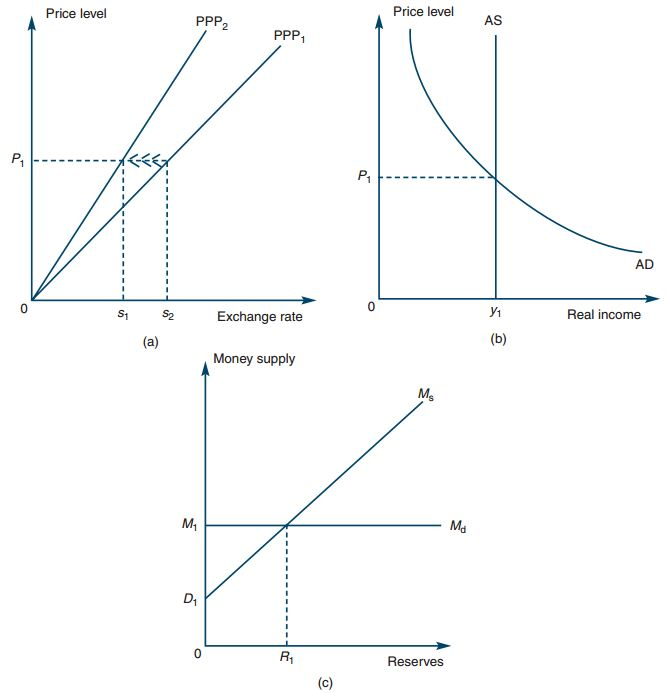
\includegraphics[scale=0.4]{fig/boptheory/lec08-25.JPG}

\end{figure}

\end{frame}

\begin{frame}{Implications of the Monetary Approach}

\begin{itemize}
\item The distinctive feature of the monetary approach

\begin{itemize}
\item money market disequilibrium is seen as a crucial factor in provoking
balance of payments disequilibrium. 
\end{itemize}
\item The core of the monetary approach

\begin{itemize}
\item The demand for money function is a stable and predictable function
of relatively few variables. 
\end{itemize}
\item Major implications

\begin{itemize}
\item In a fixed exchange-rate regime the authorities have to accept a loss
of control over their domestic monetary policy as the price of fixing
the exchange rate. 
\item It is irrelevant whether the change in the money supply results from
an OMO or an FXO.
\end{itemize}
\end{itemize}
\end{frame}

\begin{frame}{Empirical Evidence}




\begin{columns}[onlytextwidth]
\begin{column}{0.4\textwidth}
\begin{itemize}
\item Offset coefficient

\begin{itemize}
\item Measures the extent to which an increase in the domestic component
of the money base leads to a fall in reserves of a like amount in
a fixed exchange rate regime
\end{itemize}
\end{itemize}

\end{column}
\begin{column}{0.6\textwidth}
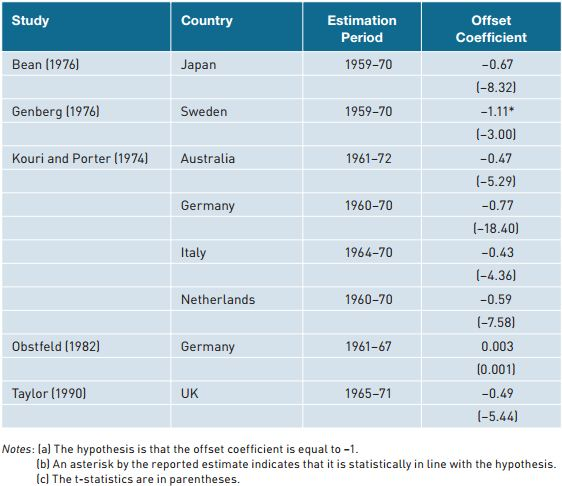
\includegraphics[width=\columnwidth]{fig/boptheory/lec08-26}
\end{column}
\end{columns}

\end{frame}

\begin{frame}{Criticisms of the Monetary Appoach}

\begin{itemize}
\item Some monetarists argue that an increase in the domestic money supply
might not be reflected exclusively in an equivalent \textbf{\textcolor{red}{fall
in the reserves}} under fixed exchange rates. (供给曲线不再是无弹性的)
\item Some critics have argued that to regard the balance of payments as
a monetary phenomenon is only true in the sense that the balance of
payments measures \textbf{\textcolor{red}{monetary flows between domestic
and foreign residents}}. 
\item Another criticism of the monetary approach is that no attention is
paid to the\textbf{\textcolor{red}{{} composition of a deficit and surplus}}. 
\end{itemize}

\end{frame}





\end{document}
